\documentclass[border=2pt]{standalone}
\usepackage{tikz}
\usetikzlibrary{positioning,arrows.meta,fit,calc}
\usepackage{times}\usepackage{bm}
\begin{document}
\footnotesize
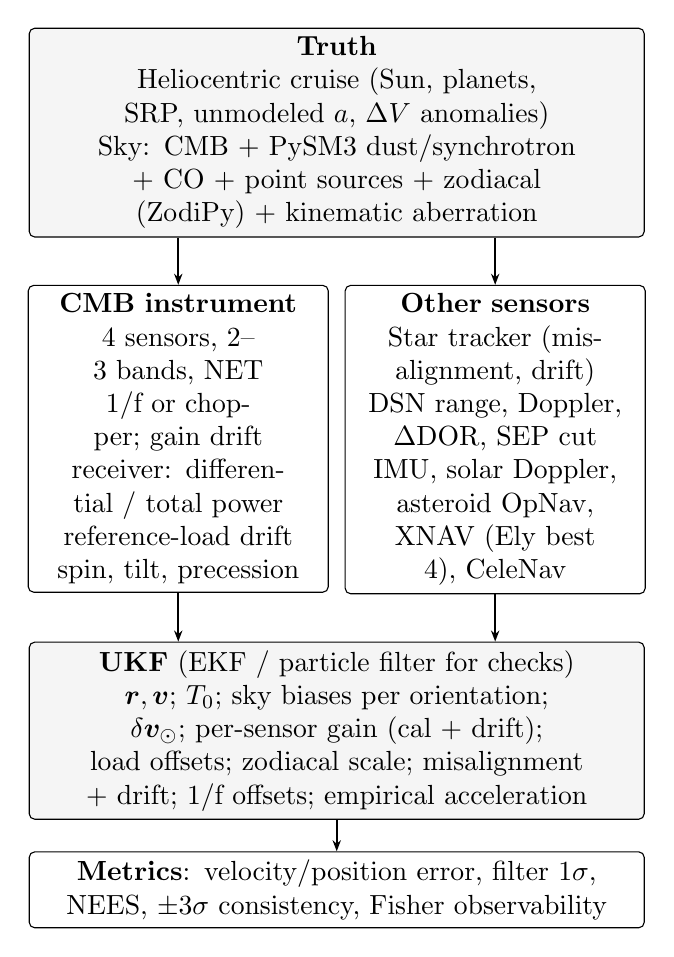
\begin{tikzpicture}[
  box/.style={draw, rounded corners=2pt, align=center, inner sep=3pt, text width=#1},
  box/.default=3.6cm,
  arr/.style={-{Stealth[length=4pt]}, thick}]
\node[box=7.6cm, fill=gray!8] (truth) {\textbf{Truth}\\ Heliocentric cruise (Sun, planets, SRP, unmodeled $a$, $\Delta V$ anomalies)\\
Sky: CMB + PySM3 dust/synchrotron + CO + point sources + zodiacal (ZodiPy) + kinematic aberration};
\node[box, anchor=north east] (inst) at ($(truth.south)+(-0.1,-6mm)$) {\textbf{CMB instrument}\\ 4 sensors, 2--3 bands, NET\\ 1/f or chopper; gain drift\\ receiver: differential / total power\\ reference-load drift\\ spin, tilt, precession};
\node[box, anchor=north west] (aux) at ($(truth.south)+(0.1,-6mm)$) {\textbf{Other sensors}\\ Star tracker (misalignment, drift)\\ DSN range, Doppler, $\Delta$DOR, SEP cut\\ IMU, solar Doppler, asteroid OpNav,\\ XNAV (Ely best 4), CeleNav};
\node[box=7.6cm, anchor=north, fill=gray!8] (ukf) at ($(truth.south |- aux.south)+(0,-6mm)$) {\textbf{UKF} (EKF / particle filter for checks)\\
$\bm{r},\bm{v}$; $T_0$; sky biases per orientation; $\delta\bm{v}_\odot$; per-sensor gain (cal + drift);\\
load offsets; zodiacal scale; misalignment + drift; 1/f offsets; empirical acceleration};
\node[box=7.6cm, below=4mm of ukf] (out) {\textbf{Metrics}: velocity/position error, filter $1\sigma$, NEES, $\pm3\sigma$ consistency, Fisher observability};
\draw[arr] (inst.north |- truth.south) -- (inst.north);
\draw[arr] (aux.north |- truth.south) -- (aux.north);
\draw[arr] (inst.south) -- (inst.south |- ukf.north);
\draw[arr] (aux.south) -- (aux.south |- ukf.north);
\draw[arr] (ukf) -- (out);
\end{tikzpicture}
\end{document}
